\documentclass[11pt]{article}
\date{April 26, 2018}
\usepackage{pgf-pie}
\usepackage{pgfplots}
\pgfplotsset{compat=1.13}
\usepackage{pgfplotstable}
\usetikzlibrary{patterns}
\usepackage[section]{placeins}
\usetikzlibrary{arrows,shadows}
\usepackage[utf8]{inputenc}
\title{My title}
\author{John Doe\\\\Associate Survey Branch Manager}

\begin{document}
\maketitle{}
\section*{Introduction}
This report has been automatically generated.


\clearpage{}
\section{Aèbc?}

\label{sec:9}


\begin{figure}[h!]
    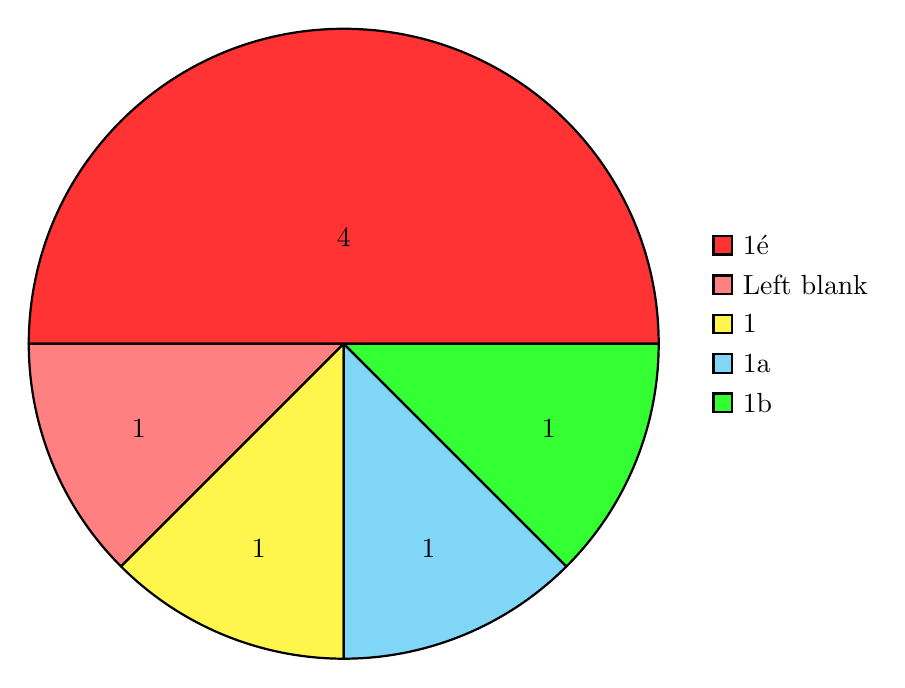
\begin{tikzpicture}
        \pie[radius=4,color={red!80, red!50, yellow!70, cyan!50, green!80},sum=auto,text=legend]{
            4/1é,
            1/Left blank,
            1/1,
            1/1a,
            1/1b
        }
    \end{tikzpicture}
    \caption{\label{figure:q9-1}Repartition of answers for the question 'Aèbc?' with '1é' standing for '1e' or '1é' or '1ë'.}
\end{figure}



\clearpage{}
\section{Bècd?}

\label{sec:10}


\begin{figure}[h!]
    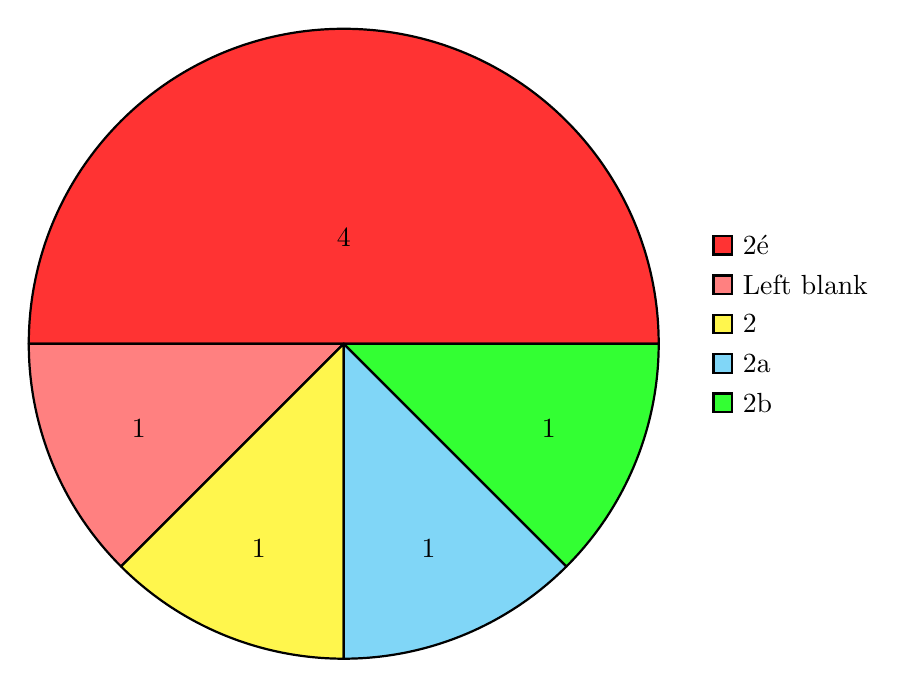
\begin{tikzpicture}
        \pie[radius=4,color={red!80, red!50, yellow!70, cyan!50, green!80},sum=auto,text=legend]{
            4/2é,
            1/Left blank,
            1/2,
            1/2a,
            1/2b
        }
    \end{tikzpicture}
    \caption{\label{figure:q10-1}Repartition of answers for the question 'Bècd?' with '2é' standing for '2e' or '2é' or '2ë'.}
\end{figure}



\clearpage{}
\section{Cède?}

\label{sec:11}


\begin{figure}[h!]
    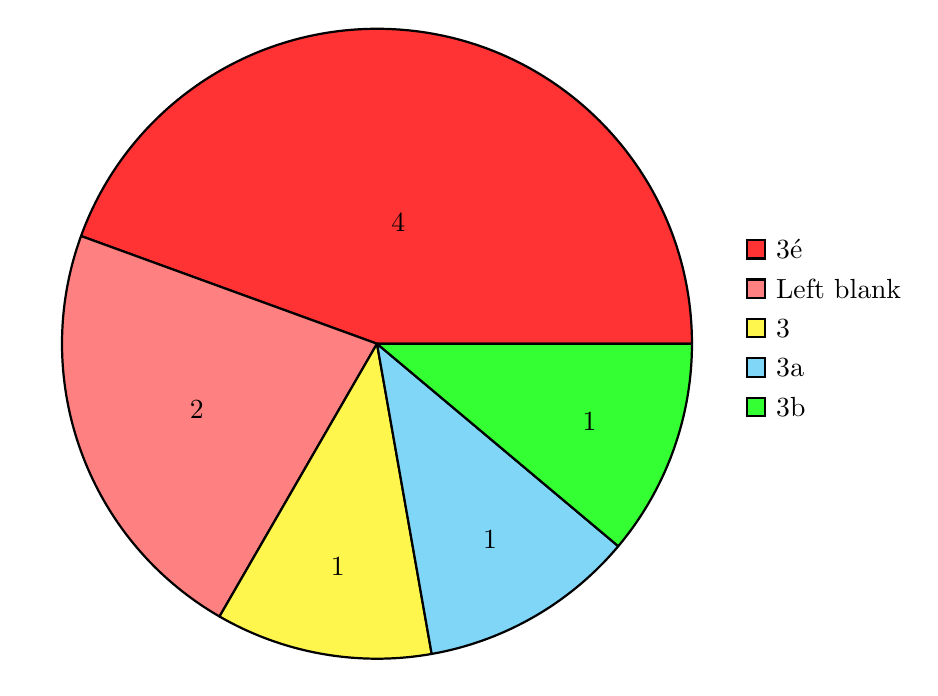
\begin{tikzpicture}
        \pie[radius=4,color={red!80, red!50, yellow!70, cyan!50, green!80},sum=auto,text=legend]{
            4/3é,
            2/Left blank,
            1/3,
            1/3a,
            1/3b
        }
    \end{tikzpicture}
    \caption{\label{figure:q11-1}Repartition of answers for the question 'Cède?' with '3é' standing for '3e' or '3é' or '3ë'.}
\end{figure}



\clearpage{}
\section{Dèef?}

\label{sec:12}

No answers for this question.

Test management footer.
\end{document}
